\documentclass[twoside]{article}
\usepackage{graphics}
\setlength{\oddsidemargin}{0.25 in}
\setlength{\evensidemargin}{-0.25 in}
\setlength{\topmargin}{-0.6 in}
\setlength{\textwidth}{6.5 in}
\setlength{\textheight}{8.5 in}
\setlength{\headsep}{0.75 in}
\setlength{\parindent}{0 in}
\setlength{\parskip}{0.1 in}

%
% The following commands set up the lecnum (lecture number)
% counter and make various numbering schemes work relative
% to the lecture number.
%
\newcounter{lecnum}
\renewcommand{\thepage}{\thelecnum-\arabic{page}}
\renewcommand{\thesection}{\thelecnum.\arabic{section}}
\renewcommand{\theequation}{\thelecnum.\arabic{equation}}
\renewcommand{\thefigure}{\thelecnum.\arabic{figure}}
\renewcommand{\thetable}{\thelecnum.\arabic{table}}

%
%% Language and font encodings
\usepackage[english]{babel}
\usepackage[utf8x]{inputenc}
\usepackage[T1]{fontenc}
\usepackage{amssymb}

%% Sets page size and margins
\usepackage[a4paper,top=3cm,bottom=2cm,left=3cm,right=3cm,marginparwidth=1.75cm]{geometry}

%
% The following macro is used to generate the header.
%
\newcommand{\lecture}[4]{
   \pagestyle{myheadings}
   \thispagestyle{plain}
   \newpage
   \setcounter{lecnum}{#1}
   \setcounter{page}{1}
   \noindent
   \begin{center}
   \framebox{
      \vbox{\vspace{2mm}
    \hbox to 6.28in { {\bf EE 382V: Social Computing
                        \hfill Fall 2018} }
       \vspace{4mm}
       \hbox to 6.28in { {\Large \hfill Lecture #1: #2  \hfill} }
       \vspace{2mm}
       \hbox to 6.28in { {\it Lecturer: #3 \hfill Scribe: #4} }
      \vspace{2mm}}
   }
   \end{center}
   \markboth{Lecture #1: #2}{Lecture #1: #2}
   %{\bf Disclaimer}: {\it These notes have not been subjected to the
   %usual scrutiny reserved for formal publications.  They may be distributed
   %outside this class only with the permission of the Instructor.}
   \vspace*{4mm}
}

%
% Convention for citations is authors' initials followed by the year.
% For example, to cite a paper by Leighton and Maggs you would type
% \cite{LM89}, and to cite a paper by Strassen you would type \cite{S69}.
% (To avoid bibliography problems, for now we redefine the \cite command.)
% Also commands that create a suitable format for the reference list.
\renewcommand{\cite}[1]{[#1]}
\def\beginrefs{\begin{list}%
        {[\arabic{equation}]}{\usecounter{equation}
         \setlength{\leftmargin}{2.0truecm}\setlength{\labelsep}{0.4truecm}%
         \setlength{\labelwidth}{1.6truecm}}}
\def\endrefs{\end{list}}
\def\bibentry#1{\item[\hbox{[#1]}]}

%Use this command for a figure; it puts a figure in wherever you want it.
%usage: \fig{NUMBER}{SPACE-IN-INCHES}{CAPTION}
\newcommand{\fig}[3]{
			\vspace{#2}
			\begin{center}
			Figure \thelecnum.#1:~#3
			\end{center}
	}


% **** IF YOU WANT TO DEFINE ADDITIONAL MACROS FOR YOURSELF, PUT THEM HERE:

%% Useful packages
\usepackage{amsmath}
\usepackage{graphicx}
\usepackage[colorinlistoftodos]{todonotes}
\usepackage[colorlinks=true, allcolors=blue]{hyperref}



\begin{document}
%FILL IN THE RIGHT INFO.
%\lecture{**LECTURE-NUMBER**}{**DATE**}{**LECTURER**}{**SCRIBE**}
\lecture{2}{August 25}{Vijay Garg}{Swapna M Mukrappilly}
%\footnotetext{These notes are partially based on those of Nigel Mansell.}


\section{Posets (Partially Ordered Sets)}

A partially ordered set is a set P equipped with a binary relation $\leq$  which is a partial order on X.   $$P = (X, \leq)$$
\begin{flushleft} X: Any set. \end{flushleft}
 \begin{flushleft}The relation $\leq$ is \textbf{reflexive}, \textbf{transitive}, \textbf{antisymmetric} relation. \end{flushleft}
 \begin{flushleft}For all a,b,c $\in\mathbb{X}$ it must satisfy,\end{flushleft}
 \begin{itemize}
\item a $\leq$ a (reflexivity: every element is related to itself)
\item  If a $\leq$ b and b $\leq$ a, then a = b (antisymmetry: two distinct elements cannot be related in both directions)
\item If a $\leq$ b and b $\leq$ c, then a $\leq$ c (transitivity: if a first element is related to second element and that element is related to a third element, then the first element is related to the third element) \end{itemize}

\section{Chains and Antichains}

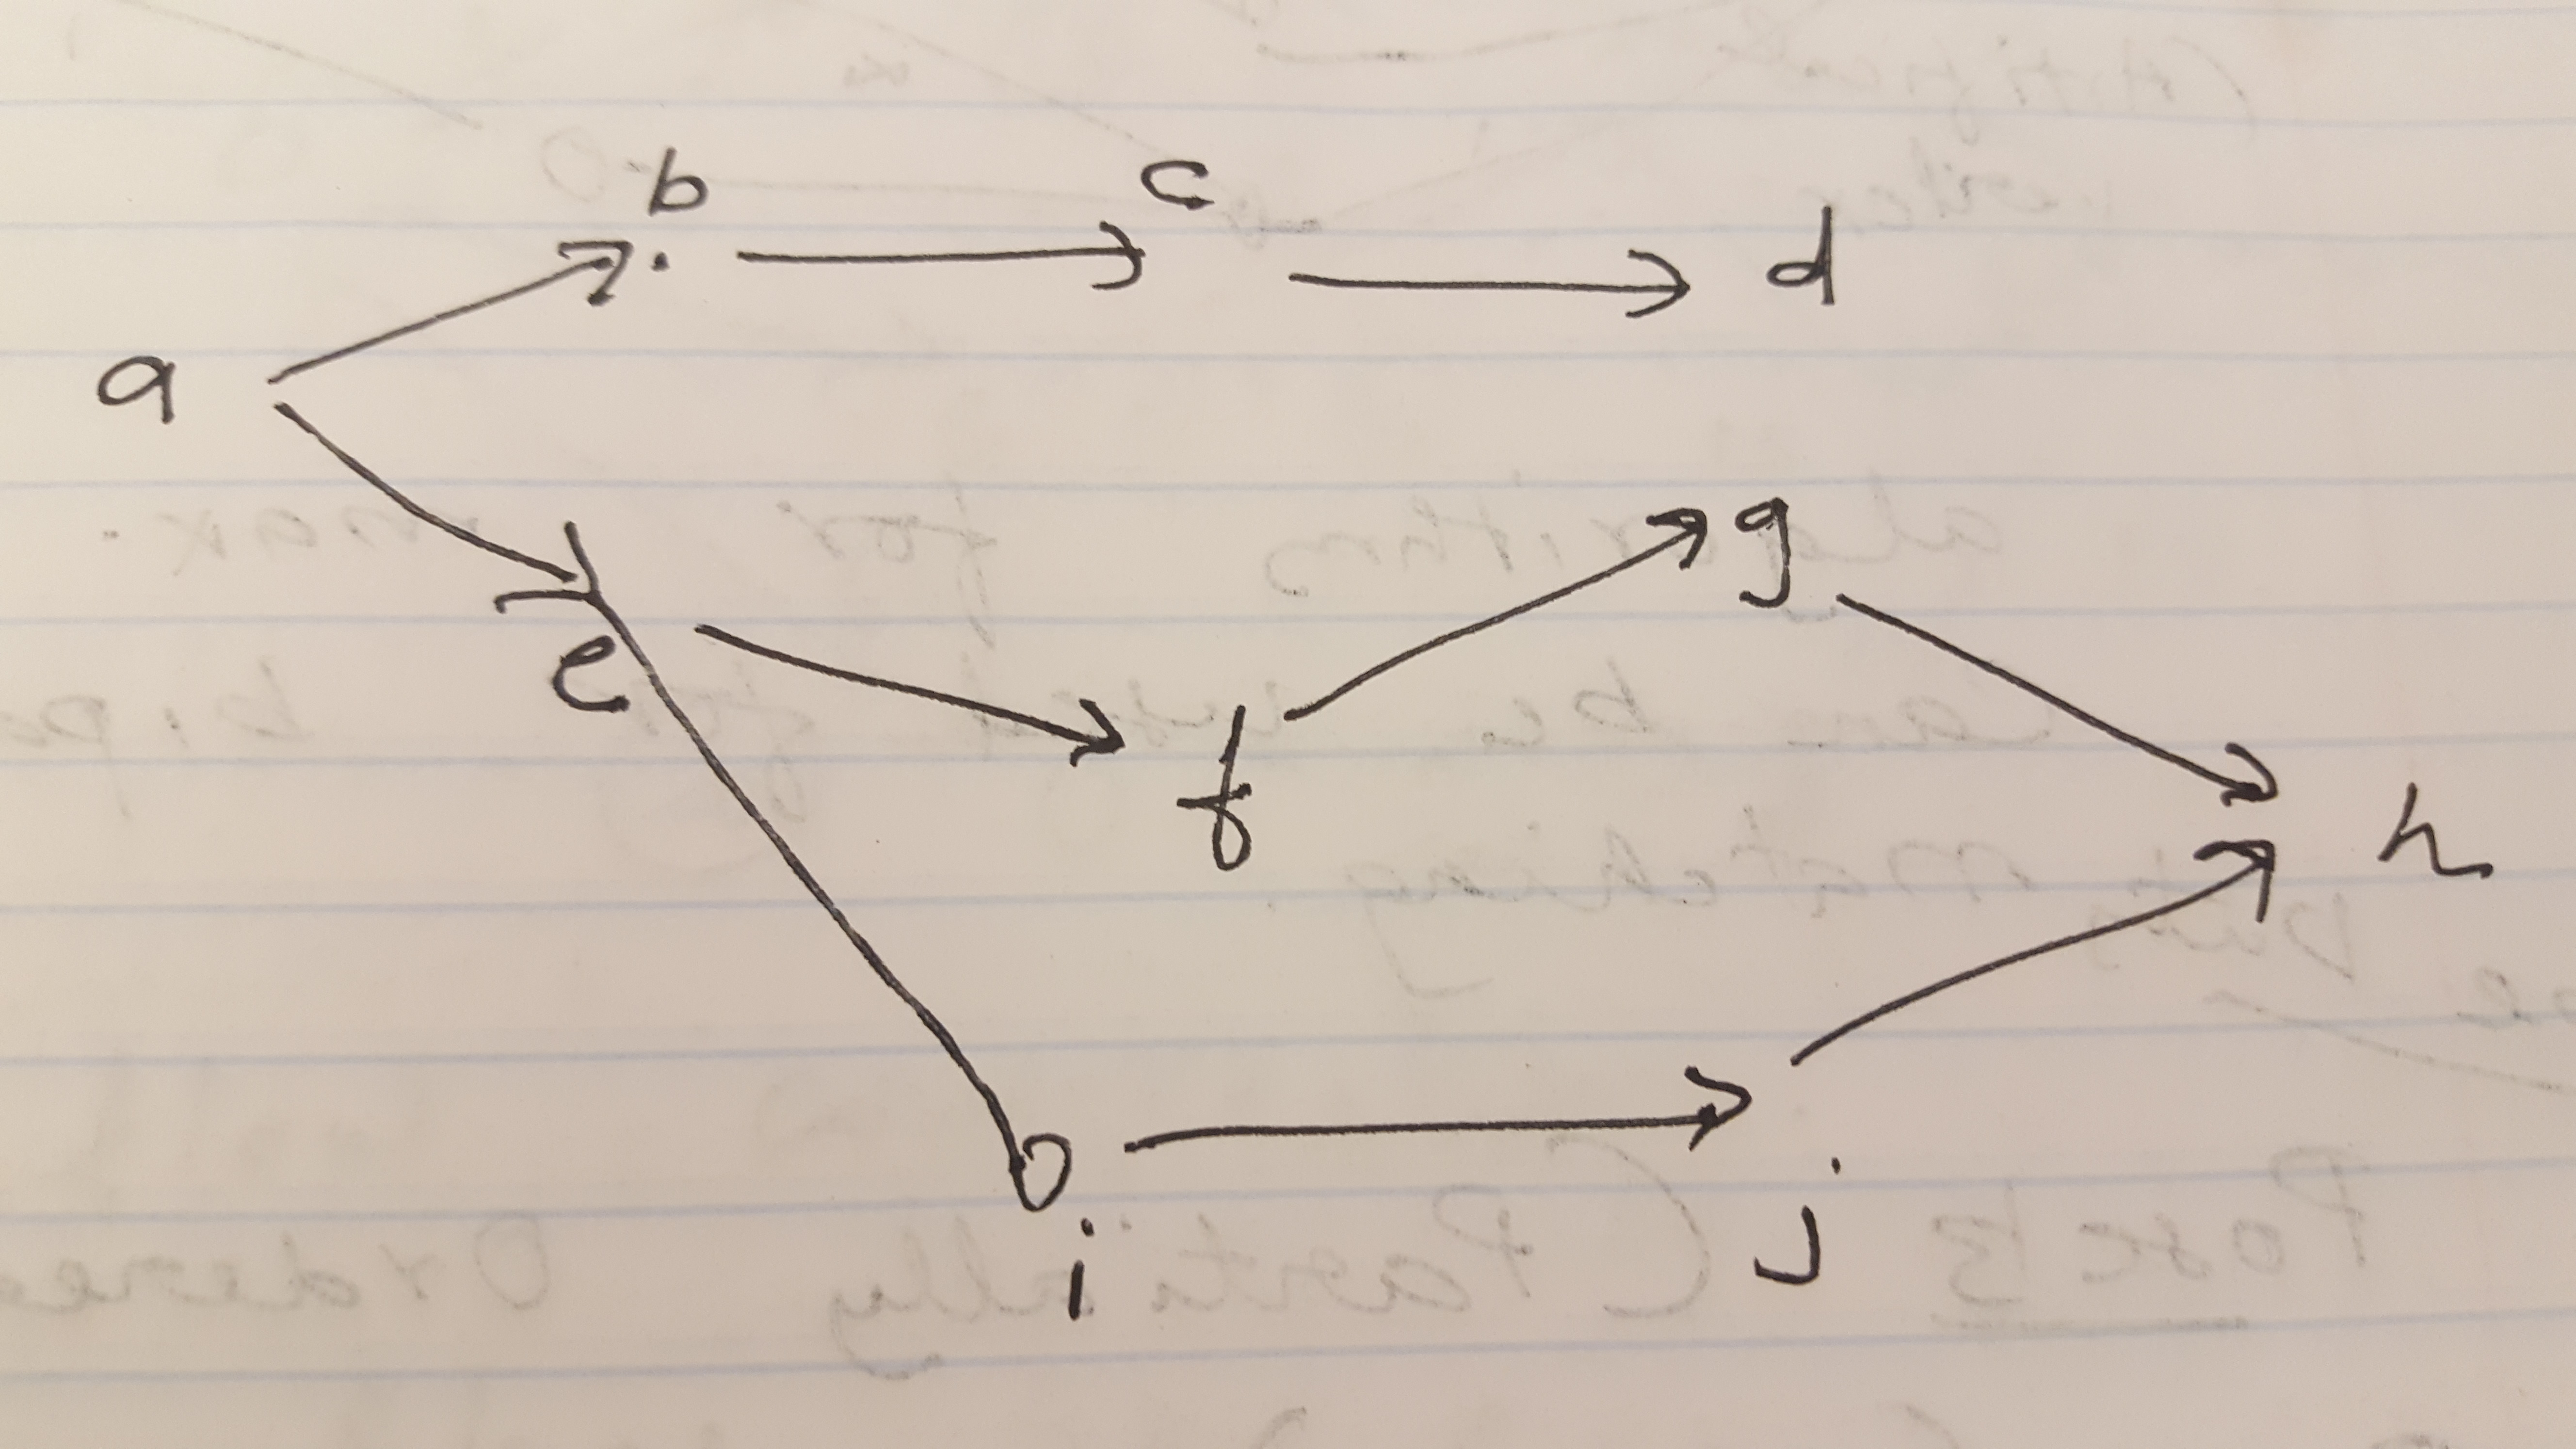
\includegraphics[width=\textwidth]{20180829_111407_001.jpg}
$C \subseteq X$ is a chain if,
$$\forall x,y \in C,  \quad    (x \leq y)  \quad or  \quad (y \leq x)$$


\begin{flushleft}In the above figure, \{a,b,c,d\} is a chain.\end{flushleft}
\begin{flushleft}
$A \subseteq X $ is an antichain if,
$$ \forall x,y \in A, \quad (x \nleq y) \wedge (y \nleq x)$$
\end{flushleft}

\begin{flushleft} In the above figure, \{c,f,i\} is an antichain.\end{flushleft}

\section{Dilworth's Theorem}

Dilworth's theorem, also called min-max theorem states that,
\begin{flushleft}
Minimum number of chains required to cover the poset = maximum sized antichain.  \end{flushleft}

\section{Answers to problems on Matching }
\begin{flushleft}\textbf{Exercise 1-1}\end{flushleft}
\begin{flushleft}
\textsl{There exists an augmenting path in G with respect to M iff there exists a directed path in D between an exposed vertex in A and an exposed vertex in B}
\end{flushleft}
\begin{flushleft} Prove the above claim\end{flushleft}
\begin{flushleft} Answer:\end{flushleft}

\begin{flushleft}Proof:-\end{flushleft}
\begin{flushleft}Let us consider an a maximal matching M and a maximum matching M*. The symmetric difference D is a subgraph between M and M∗, $D = M \bigoplus M*$  \end{flushleft}
\begin{flushleft} As both M and M∗ are matchings, each vertex in D can have degree not greater than 2, because it can be adjacent to at most one edge from each matching. If a vertex has degree equal to 2, then it is adjacent to one edge from M and one edge from M∗. Therefore, all the cycles and paths are alternating but cycles can only be even-length.\end{flushleft}
\begin{flushleft} As |M∗| > |M| and $ D = M∗ \bigoplus  M = (M∗ ∪ M) \backslash (M∗ ∩ M) $ it is also true that $|D ∩ M∗| > |D ∩ M|$, meaning that there are more edges from M* than M in D. Since cycles can only be even length, the augmenting path can only be odd-length paths that start and end with edges from M∗. Hence an augmenting path has to be a directed path and not a cycle. \end{flushleft}
\begin{flushleft} If the vertices in A and B were not exposed, there would already been  an edge between A and B resulting in a non-disjoint set. \end{flushleft}
\begin{flushleft} Thus we can prove that an augmenting path can exist if and only if there is a directed path between an exposed vertex in A and an exposed vertex in B \end{flushleft}
\begin{flushleft}\textbf{Exercise 1-2}\end{flushleft}
\begin{flushleft}An edge cover of a graph G = (V, E) is a subset of R of E such that every vertex of V is incident to at least one edge in R. Let G be a bipartite graph with no isolated vertex.  Show that the cardinality of the minimum edge cover R∗ of G is equal to |V | minus the cardinality of the maximum matching M∗ of G. 
Is this true also for non-bipartite graphs? \end{flushleft}
\begin{flushleft} Answer:\end{flushleft}
\begin{flushleft} 
Let  $\nu(G)$ be the size of the maximum matching M*. \end{flushleft}
\begin{flushleft} Let n =|V| be the number of vertices in the  graph G.\end{flushleft}
\begin{flushleft}We will construct an edge cover  as follows,\end{flushleft}
\begin{flushleft}
A maximum matching M* covers $2\nu(G)$ vertices.Since there are no isolated vertices,  the vertices that are left uncovered =  $n- 2\nu(G)$. 
\end{flushleft}
\begin{flushleft}If we use one edge to cover one vertex, the total size of the edge cover |R*|, $\rho(G)$\end{flushleft}
$$\leq \nu(G) + n - 2\nu(G)$$
$$\leq n- \nu(G) $$
$$\rho(G) + \nu(G) \leq n \quad  \quad ..............(1)$$ 
\begin{flushleft} Let R* be the minimum edge cover. Since removing any edge from R* yields an uncovered vertex, each edge has an endpoint of degree 1 in (V, R*)  \end{flushleft}
\begin{flushleft} This implies that (V, R*) consists of disjoint sets. The number of components in (V, R*) $$= |V| - |R*| $$
$$= n -\rho(G) $$
Now we construct a matching M of size $n-\rho(G)$ by choosing one edge from each disjoint set in (V, R*)
 \end{flushleft}
 \begin{flushleft} Maximum matching $|M*| \geq n - \rho(G)$  \end{flushleft}
 $$ \nu(G) \geq n - \rho(G) $$
 $$ \nu(G) + \rho(G) \geq n \quad \quad .............(2) $$
 \begin{flushleft} From (1) and (2) we get, \end{flushleft}
 $$ \nu(G) + \rho(G) = n $$
\begin{flushleft} The result is true for non-bipartite graphs too. \end{flushleft}


\begin{flushleft}\textbf{Exercise 1-3}\end{flushleft}
\begin{flushleft} Show that in any graph G= (V,E) (not necessarily bipartite), the size of any maximal matching is at least half the size of a maximum matching M* \end{flushleft}
\begin{flushleft} Answer:\end{flushleft}
\begin{flushleft}
Consider a maximum matching M* of size $\alpha(G)$. For every edge in M*, at least one endpoint of the edge must be present in any maximal matching(or the edge can be added to the matching, and hence it won't be maximal). Hence, the number of vertices covered by any maximal matching must at least be $\mid M* \mid = \alpha(G)$. Since an edge in the matching can cover at most two vertices, the number of edges in the maximal matching must be $\alpha(G) /2$.
\end{flushleft}

\end{document}